\loai{Tính suất điện động khi biết L}
\begin{vidu}%[2P5-5.1K][Loai1]
Một ống dây có hệ số tự cảm $L = 0,1$ H, cường độ dòng điện qua ống dây giảm đều đặn từ 2 A về 0 trong khoảng thời gian là 4 s. Suất điện động tự cảm xuất hiện trong ống trong khoảng thời gian đó là
\choice
{0,03 V}
{0,04 V}
{0,06 V}
{\True 0,05 V}
\loigiai{
Áp dụng công thức tính độ lớn của suất điện động tự cảm là: $e = L\left| {\dfrac{\Delta I}{\Delta t}} \right| = 0,1.\left| {\dfrac{0 - 2}{4}} \right| = 0,05$ V.
}
\end{vidu}
\loai{Tính hệ số tự cảm}
\begin{vidu}%[2P5-5.1K][Loai2]
Dòng điện qua một ống dây không có lõi sắt biến đổi đều theo thời gian, trong 0,01 s cường độ dòng điện tăng đều từ 1 A đến 2 A thì suất điện động tự cảm trong ống dây là 20 V. Tính hệ số tự cảm của ống dây.
\choice
{0,1 H}
{\True 0,2 H}
{0,3 H}
{0,2 H}
\loigiai{
Hệ số tự cảm của ống dây là: $L=\dfrac{e_{tc}.\Delta t}{\Delta I}=\dfrac{20.(2-1)}{0,01}=0,2\;H$.
}
\end{vidu}
\loai{Tính biến thiên cường độ dòng điện}
\begin{vidu}%[2P5-5.1K][Loai3]
Một ống dây có độ tự cảm 0,4 H. Trong khoảng thời gian 0,04 s, suất điện động tự cảm xuất hiện ở ống dây là 50 V. Độ biến thiên cường độ dòng điện trong khoảng thời gian đó là
\choice
{4,5 A}
{2,5 A}
{\True 5 A}
{7,5 A}
\loigiai{
Độ biến thiên cường độ dòng điện trong khoảng thời gian 0,04 s là: $\left|{\Delta I}\right|=\dfrac{e_{tc}.\Delta t}{L}=\dfrac{50.0,04}{0,4}=5\ A$
}
\end{vidu}
\loai{Tính suất điện động khi biết cấu trúc mạch}
\begin{vidu}%[2P5-5.1K][Loai4]
Một ống dây dài 40 cm, đường kính 4 cm có 400 vòng dây quấn sát nhau. Ống dây có dòng điện 1 A chạy qua. Sau khi ngắt ống dây ra khỏi nguồn điện, biết từ thông qua ống dây giảm đều từ giá trị ban đầu đến 0 trong khoảng thời gian 0,01 s. Suất điện động tự cảm trong ống dây là
\choice
{0,054 V}
{\True 0,063 V}
{0,039 V}
{0,051 V}
\loigiai{
\begin{itemize}
\item Hệ số tự cảm của ống dây là:  $L=4\pi.10^{-7}.n^2.V=4\pi.10^{-7}.\left({\dfrac{400}{0,4}}\right)^2.0,4.\dfrac{\pi.0,{04}^2}{4}=6,3.10^{-4}\ H$.
\item Suất điện động tự cảm trong ống dây là:  $e_{tc}=L.\left|{\dfrac{\Delta I}{\Delta t}}\right|=6,3.10^{-4}.\dfrac{1}{0,01}=0,063\ V$.
\end{itemize}
}
\end{vidu}
\loai{Cho biểu thức dòng điện}
\begin{vidu}%[2P5-5.1K][Loai6]
Một dòng điện trong ống dây phụ thuộc vào thời gian theo biểu thức $I=0,4.(5-t)$; I tính bằng ampe, t tính bằng giây. Ống dây có hệ số tự cảm $L = 0,005\ H$. Tính suất điện động tự cảm trong ống dây.
\choice
{0,001 V}
{\True 0,002 V}
{0,003 V}
{0,004 V}
\loigiai{
Ta có: $e=L\left|{\dfrac{\Delta I}{\Delta t}}\right|=L\left|{\dfrac{I_{\left({t_2}\right)}-I_{\left({t_1}\right)}}{t_2-t_1}}\right|=L\left|{\dfrac{0,4\left({5-t_2}\right)-0,4\left({5-t_1}\right)}{t_2-t_1}}\right|=L\left|{\dfrac{-0,4\left({t_2-t_1}\right)}{t_2-t_1}}\right|=0,4L.$
}
\end{vidu}
\loai{Đồ thị}
\begin{vidu}%[2P5-5.1K][Loai7]
immini[thm]{
Một ống dây được quấn với mật độ 2000 vòng/mét. Ống dây có thể tích 500 $cm^3$. Ống dây được mắc vào một mạch điện. Sau khi đóng công tắc, dòng điện trong ống biến đổi theo thời gian như đồ thị trên hình vẽ. Suất điện động tự cảm trong ống từ sau khi đóng công tắc đến thời điểm 0,05 s là
\choice
{1 V}
{0,5 V}
{\True 0,25 V}
{3 V}}{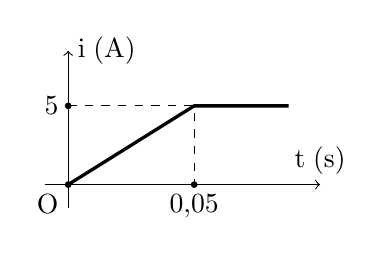
\begin{tikzpicture}
\coordinate (o) at (0,0);
\draw [->](0,-0.3)--++(90:2)node[right]{\normalsize{\bth{i\;(A)}}};
\draw [->](-0.3,0)--++(0:3.5)node[above]{\normalsize{\bth{t\;(s)}}};
\draw[very thick](0,0)--(1.6,1)--(2.8,1);
\draw[dashed](0,1)--(1.6,1)--(1.6,0);
\filldraw[black] (0,0)circle(1pt)node[below left]{\normalsize{\bth{O}}};
\filldraw[black] (1.6,0)circle(1pt)node[below]{\normalsize{\bth{0,05}}};
\filldraw[black] (0,1)circle(1pt)node[left]{\normalsize{\bth{5}}};
\end{tikzpicture}}
\loigiai
{
\begin{itemize}
\item Hệ số tự cảm: $L = 4\pi .{10^{- 7}}.{n^2}.V$
\item Suất điện động tự cảm: $e = L\dfrac{{\left| {\Delta I} \right|}}{{\Delta t}}=0,25\ V$.
\end{itemize}
}
\end{vidu}
\loai{Tổng hợp}

